% Für Seitenformatierung

\documentclass[DIV=15]{scrartcl}

% Zeilenumbrüche

\parindent 0pt
\parskip 6pt

% Für deutsche Buchstaben und Synthax

\usepackage[ngerman]{babel}

% Für Auflistung mit speziellen Aufzählungszeichen

\usepackage{paralist}

% zB für \del, \dif und andere Mathebefehle

\usepackage{amsmath}
\usepackage{commath}
\usepackage{amssymb}

% Für \SIunit[]{} und \num in deutschem Stil

\usepackage[output-decimal-marker={,}]{siunitx}

% Schriftart und encoding

\usepackage[utf8]{inputenc}
\usepackage[charter, greekuppercase=italicized]{mathdesign}
\usepackage{beramono}

% Für \sfrac{}{}, also inline-frac

\usepackage{xfrac}

% Für Einbinden von pdf-Grafiken

\usepackage{graphicx}

% Umfließen von Bildern

\usepackage{floatflt}

% Für Links nach außen und innerhalb des Dokumentes

\usepackage{hyperref}

% Für weitere Farben

\usepackage{color}

% Für Streichen von z.B. $\rightarrow$

\usepackage{centernot}

% Für Befehl \cancel{}

\usepackage{cancel}

% Für Layout von Links

\hypersetup{
	citecolor=black,
	colorlinks=true,
	linkcolor=black,
	urlcolor=blue,
}

% Verschiedene Mathematik-Hilfen

\newcommand \e[1]{\cdot10^{#1}}
\newcommand\p{\partial}

\newcommand\half{\frac 12}
\newcommand\shalf{\sfrac12}

\newcommand\skp[2]{\left\langle#1,#2\right\rangle}
\newcommand\mw[1]{\left\langle#1\right\rangle}
\newcommand \eexp[1]{\mathrm{e}^\del{#1}}
\newcommand \dexp[1]{\exp\del{#1}}

% Nabla und Kombinationen von Nabla

\renewcommand\div[1]{\skp{\nabla}{#1}}
\newcommand\rot{\nabla\times}
\newcommand\grad[1]{\nabla#1}
\newcommand\laplace{\triangle}
\newcommand\dalambert{\mathop{{}\Box}\nolimits}

%Für komplexe Zahlen

\newcommand \ii{\mathrm i}
\renewcommand{\Im}{\mathop{{}\mathrm{Im}}\nolimits}
\renewcommand{\Re}{\mathop{{}\mathrm{Re}}\nolimits}

%Für Bra-Ket-Notation

\newcommand\bra[1]{\left\langle#1\right|}
\newcommand\ket[1]{\left|#1\right\rangle}
\newcommand\braket[2]{\left\langle#1\left.\vphantom{#1 #2}\right|#2\right\rangle}
\newcommand\braopket[3]{\left\langle#1\left.\vphantom{#1 #2 #3}\right|#2\left.\vphantom{#1 #2 #3}\right|#3\right\rangle}


\setcounter{section}{0}
\renewcommand\thesection{H\,7.\arabic{section}}
\renewcommand\thesubsection{\thesection.\alph{subsection}}

\title{physik521: Übungsblatt 07}
\author{%
    Lino Lemmer \\ \small{\texttt{lino.lemmer@uni-bonn.de}}
    \and
    Martin Ueding \\ \small{\texttt{mu@martin-ueding.de}}
    \and
    Paul Manz \\ \small{\texttt{p.m@uni-bonn.de}}
}

\begin{document}
\maketitle
\section{Zweiatomiges Molekül}

\subsection{Schwingung}

Die möglichen Energien eines harmonischen Oszillators sind gegeben durch
\begin{align*}
    E_n^\text{Ozs} &= \hbar\omega\del{n+\half}.
    \intertext{%
        Die kanonische Zustandssumme für $N$ unabhängige Oszillatoren ist das
        Produkt aller einzelnen, wegen der Unabhängigkeit gleichen,
        Zustandssummen. Mit $\beta = \del{k_\text{B}T}^{-1}$ erhält man
    }
    \del{Z_\text{C}^\text{Ozs}}^N &= \del{\sum_n^N\dexp{-\beta
    E_n^\text{Osz}}}^N \\
    &= \del{\sum_n^N \dexp{-\beta\hbar\omega \del{n+\half}}}^N \\
    &= \del{\dexp{-\half\hbar\omega\beta}\sum_n^N\dexp{-\hbar\omega\beta n}}^N
    \intertext{%
        Die Summe kann man mit einer geometrischen Reihe Umschreiben.
    }
    &= \del{\frac{\dexp{-\half\hbar\omega\beta}}
    {1-\dexp{-\hbar\omega\beta}}}^N\\
    &= \del{\frac{1}{2\sinh\del{-\half\hbar\omega\beta}}}^N
    \intertext{%
        Die innere Energie des Systems ist, auch hier wegen der Unabhängigkeit,
        die Summe aller mittleren Energien. Bei $N$ Molekülen erhalten wir daher
    }
    U^\text{Osz} &= N \mw{E} \\
    &= \frac{N}{Z_\text{C}^\text{Osz}}\sum_n E_n^\text{Osz} \dexp{-\beta E_n} \\
    &= -\frac{N}{Z_\text{C}^\text{Osz}} \dpd{}{\beta}
    \underbrace{ \sum_n \dexp{-\beta E_n}}_{=Z_\text{C}^\text{Osz}} \\
    &= -N \dpd{}{\beta}\log\del{Z_\text{C}^\text{Osz}} \\
    &= -N \dpd{}{\beta}\log\del{\frac{1}{2\sinh\del{\half\hbar\omega\beta}}} \\
    &= N\dpd{}{\beta}\log\del{2\sinh\del{\half\hbar\omega\beta}} \\
    &= N\frac{\hbar\omega}{2}\coth\del{\half\hbar\omega\beta}.
    \intertext{%
        Die spezifische Wärme ist definiert als
    }
    C_V^\text{Osz} &= \dpd{U^\text{Osz}}{T} \\
    &= N\frac{\hbar\omega}{2} \dpd{}{T} \coth\del{\half\hbar\omega\beta} \\
    &= N\frac{\hbar\omega}{2} \dpd{}{T}
    \coth\del{\frac{\hbar\omega}{2k_\text{B}T}} \\
    &= N\frac{\del{\hbar\omega}^2}{4k_\text{B}}
    \frac{1}{T^2\sinh^2\del{\frac{\hbar\omega}{2k_\text{B}T}}} \\
    &= Nk_\text{B}\del{\frac{\hbar\omega}{2k_\text{B}T}}^2
    \frac{1}{\sinh^2\del{\frac{\hbar\omega}{2k_\text{B}T}}} \\
\end{align*}
Das Verhalten der spezifischen Wärme für $k_\text{B}T\ll\hbar\omega$ ist in
Abbildung~\ref{fig:C_V_Osz_ll} und für $k_\text{B}T\gg\hbar\omega$ in
Abbildung~\ref{fig:C_V_Osz_gg} gezeigt.

\begin{figure}
    \centering
    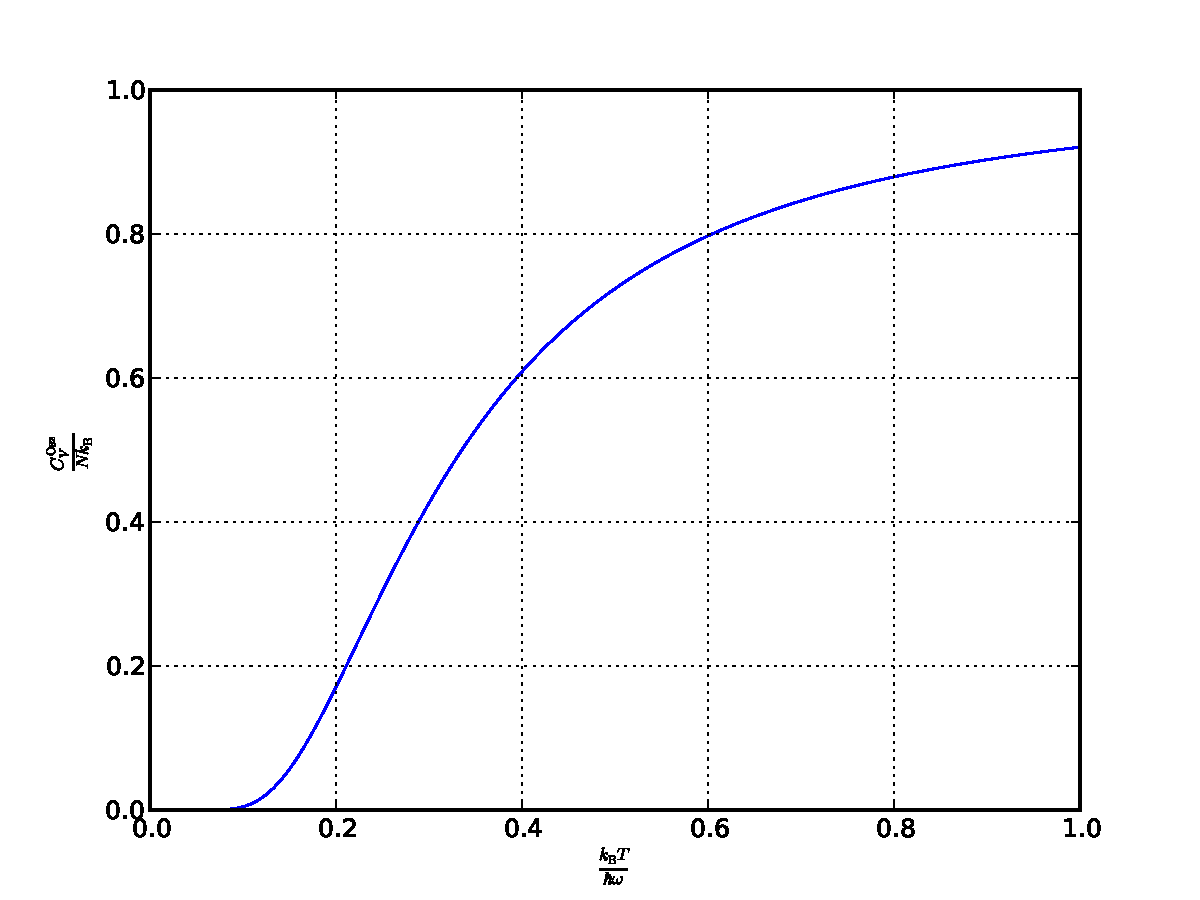
\includegraphics[width=\textwidth]{C_V_Osz_ll.pdf}
    \caption{Verhalten der spezifischen Wärme}
    \label{fig:C_V_Osz_ll}
\end{figure}

\begin{figure}
    \centering
    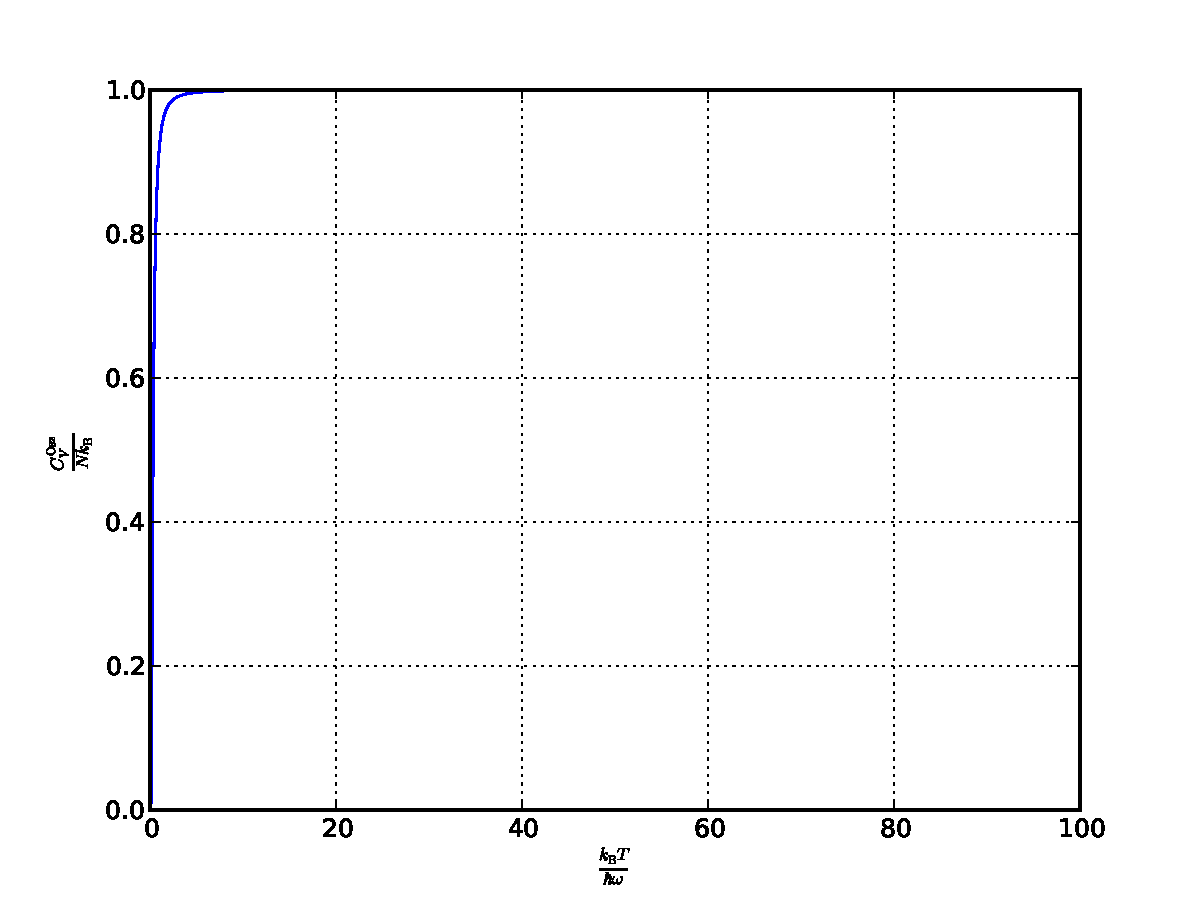
\includegraphics[width=\textwidth]{C_V_Osz_gg.pdf}
    \caption{Verhalten der spezifischen Wärme}
    \label{fig:C_V_Osz_gg}
\end{figure}

\subsection{Rotation}

\begin{align*}
    E_l^\text{Rot} &= \frac{J^2}{2I} \\
                   &= \frac{\hbar l\del{l+1}}{2I}
    \intertext{%
        Die kanonische Zustandssumme ist auch die eines einzelnen Moleküls in
        $N$-ter Potenz. Wir berechnen zunächst für ein Molekül. Da wir hier
        eigentlich über $m_l$ summieren müssten, nehmen wir für die Entartung
        einen Faktor $2l+1$ hinzu:
    }
    Z_C^\text{Rot} &= \sum_l^N \del{2l+1}\dexp{-\beta E_l^\text{Rot}} \\
    &= \sum_l^N \del{2l+1}\dexp{-\beta \frac{\hbar l\del{l+1}}{2I}}
    \intertext{%
        Wir schauen uns nun zwei Näherungen an. Für niedrige Temperaturen kann
        nach Euler-MacLaurin folgendes geschrieben werden
    }
    Z_C^\text{Rot} &= \num{0.5} + \int_0^\infty\!\dif l \del{2l+1}\dexp{-\beta
    \frac{\hbar l\del{l+1}}{2I}} \\
    &= \num{0.5} -\frac{2I}{\beta\hbar}\sbr{\dexp{-\beta\frac{\hbar
    l\del{l+1}}{2I}}}_0^\infty \\
    &= \num{0.5} + \frac{2I}{\beta\hbar}
    \intertext{%
        Für hohe Temperaturen benötigt man zwei Terme zusätzlich:
    }
    Z_C^\text{Rot} &= \num{0.5} + \frac{2I}{\beta\hbar} -
    \frac1{12}\dpd{}{l} \left.\del{2l+1}\dexp{-\beta \frac{\hbar
    l\del{l+1}}{2I}}\right|_{l=0} + \frac1{720}\dpd[3]{}{l}
    \left.\del{2l+1}\dexp{-\beta \frac{\hbar l\del{l+1}}{2I}}\right|_{l=0} \\
    &= \num{0.5} + \frac{2I}{\beta\hbar} -
    \frac1{12}\del{2-\frac{\beta\hbar}{2I}} + \frac
    1{720}\del{\del{\frac{\beta\hbar}{2I}}^3 -
    12\del{\frac{\beta\hbar}{2I}}^2 + 12 \frac{\beta\hbar}{2I}} \\
    &= \frac13 + \frac{2I}{\beta\hbar} + \frac1{10} \frac{\beta\hbar}{2I} -
    \frac1{60}\del{\frac{\beta\hbar}{2I}}^2 +
    \frac1{720}\del{\frac{\beta\hbar}{2I}}^3
    \intertext{%
        Analog zur inneren Energie für die Schwingung erhalten wir
    }
    U^\text{Rot} &= -N\dpd{}{\beta}\log\del{\frac13 + \frac{2I}{\beta\hbar} +
    \frac1{10} \frac{\beta\hbar}{2I} - \frac1{60}\del{\frac{\beta\hbar}{2I}}^2 +
    \frac1{720}\del{\frac{\beta\hbar}{2I}}^3 }
\end{align*}

\section{Kühlung durch adiabatische Entmagnetisierung}


\section{Polymer-Modell (Gummi)}

\end{document}

%vim: tw=79 spell spelllang=de
